% (approx. 400-800 words)
The purpose of this section is to show and explain as much as possible the results that have been obtained in different runs. In particular, it is mandatory to state that, if not specified otherwise, the following implementation choices and hyper-parameters have been used for both models:
\begin{itemize}
    \item SGD as optimizer, with learning rate set to $1$, weight decay to $10^{-6}$, and momentum to $0.9$;
    \item training batch size of $32$;
\end{itemize}
Similarly, for AWD-LSTM the following was considered:
\begin{itemize}
    \item parameter tying between the embedding dropout and the classification layer;
    \item weight initialisation using xavier\_uniform for the LSTM weights, and uniform\_ (i.e. $(-0.1, 0.1)$) for the embedding;
    \item training batch size of $32$;
    \item gradient clip to $0.25$
    \item ASGD with the same (shared) parameters of the SGD;
    \item embedding dropout of $0.1$ instead of regular dropout;
    \item locked dropout of $0.4$ between both the embedding and the classification layers;
    \item weight dropout of $0.5$ for LSTM \textit{hidden-to-hidden} weights;
    \item dropout of $0.3$ between the LSTM recurrent layers.
\end{itemize}

\subsection{Evaluation metric}
The evaluation of the model has been performed intrinsically using \textit{per word perplexity} (PP), which is defined as the exponential of the Cross Entropy, and is computed as follows:

\begin{equation}
    PP(W) = \exp{(L_{CE}(W))}
\end{equation}

where $W$ is a sequence of words, while $L_{CE}$ is the Cross Entropy Loss. Given that such computation is approximated at batch level, per word perplexity can be written as:

\begin{equation}
    PP(x, y) = \exp{\left(-\frac{1}{N} \sum^{N}_{i=1}{\sum^{C}_{j=1}{y_{ij} \log{f_{\theta}(x_{ij})}}}\right)}
\end{equation}
where $N$ is the number of elements (i.e. words) in a batch, $C$ the total number of classes (i.e. vocabulary length), $x \text{ and } y$ are the input and target words respectively, and $f_{\theta}$ is the model with weights $\theta$.

The overall objective is of course to find the best set of weights $\theta^*$ which is able to minimise the overall per word perplexity (i.e. computed on the whole dataset), namely:
\begin{equation}
    \theta^* = \text{arg min}_{\theta} PP(X, Y)
\end{equation}

Last but not least, for the perplexity computation I have removed the padding tokens to ignore irrelevant predictions.

\subsection{Results}

\begin{figure}
    \centering
    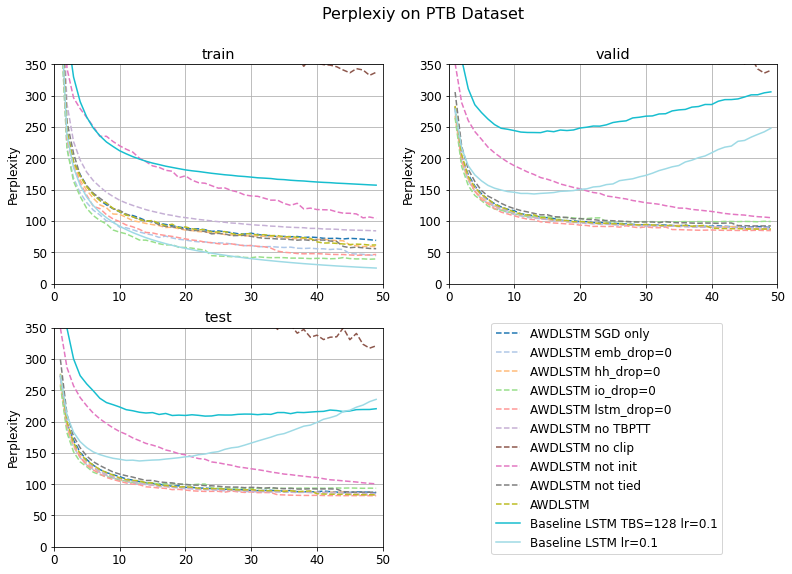
\includegraphics[scale=0.28]{assets/run_results.png}
    \vspace{-1.0em}
    \caption{Perplexity per epoch on PTB train, valid, and test sets}
    \vspace{-1.0em}
    \label{fig:results}
\end{figure}

\Cref{fig:results} shows the results of the several runs that have been performed, mostly to understand the effect of the regularisation and optimisation techniques that have been introduced.

By first analysing the \textit{Baseline}, it is possible to see how easily such model overfits, reaching astonishing performance on the training set by essentially memorising the data, but catastrophic results on the valid and test set.

Starting from such evidence, it was obvious that to improve the performance more regularisation techniques were needed. This led to the current AWD-LSTM implementation, which is explained more in detail in \Cref{sec:model}. The results obtained by considering such a model are obviously better; however, there are still some really interesting behaviours when analysing one by one the regularisation techniques.

To my surprise, I was actually very intrigued by how much performance changed whenever weight initialisation (i.e. \textit{AWDLSTM not init}) and clipping (i.e. \textit{AWDLSTM no clip}) were not performed. Of course, starting from a more favourable position leads to better results, explaining why weight initialisation is particularly important (i.e. the model converges faster and reaches a better local minimum). Instead, clipping the gradient is mandatory to avoid \textit{exploding gradient} when considering AWD-LSTM, given the fact that the shared parameters used during backpropagation start to become quite a few, causing such an undesired effect.

\begin{figure}
    \centering
    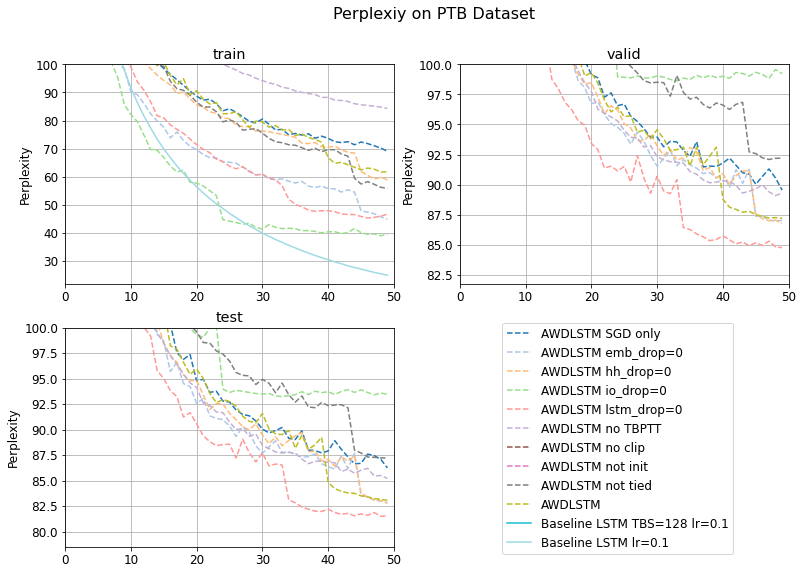
\includegraphics[scale=0.28]{assets/run_results_zoom_in.png}
    \vspace{-1.5em}
    \caption{Perplexity per epoch on PTB train, valid, and test sets (best runs details)}
    \vspace{-1.5em}
    \label{fig:results-zoom}
\end{figure}

\Cref{fig:results-zoom} shows a zoom-in of the previous image, depicting how the best techniques differ one from another in terms of performance. As it is possible to notice, they are all pretty close; however, we can see how
\begin{itemize}
\item without applying locked dropout (i.e. \textit{AWDLSTM io\_drop=0}) between both the embedding dropout and the classification layers, the model tends to overfit more on the training set, while obtaining worse performance on the validation and test set;
\item without parameters tying between the embedding and the classification layer (i.e. \textit{AWDLSTM not tied}) we achieve worse performance since the model is required to learn more parameters;
\item without ASGD (i.e. \textit{AWDLSTM SGD only}) convergence to the optimum is slower (i.e. the other runs benefit of the average).
\end{itemize}

\subsection{Error analysis}
To understand the reason why a model obtained certain performances, I tried to look at the length of the sentences that obtained better and worse results w.r.t. the average perplexity. The general idea was to find a correlation between a certain length and a possible source of error, e.g. discovering that the majority of short sentences were wrongly predicted. However, their distribution was pretty much identical in all the sets, meaning that sentences with different lengths appeared in both the splits.

\begin{figure}[!t]
    \centering
    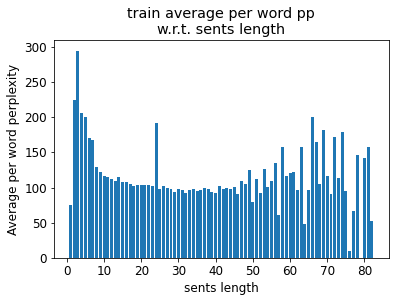
\includegraphics[scale=0.40]{assets/baseline_train_pp_per_length.png}
    \vspace{-1.0em}
    \caption{Baseline average perplexity per sentence length on the train set}
    \vspace{-1.0em}
    \label{fig:baseline-train-pp}
\end{figure}

\begin{figure}[!t]
    \centering
    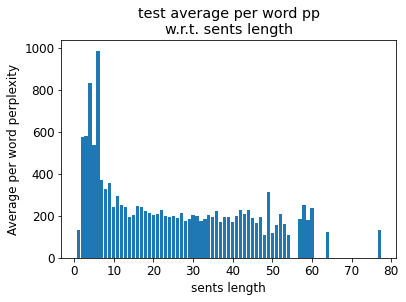
\includegraphics[scale=0.40]{assets/baseline_test_pp_per_length.png}
    \vspace{-1.0em}
    \caption{Baseline average perplexity per sentence length on the test set}
    \vspace{-1.0em}
    \label{fig:baseline-test-pp}
\end{figure}

\begin{figure}[!t]
    \centering
    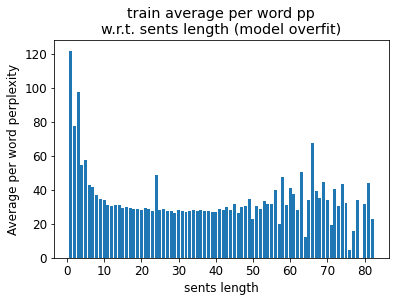
\includegraphics[scale=0.40]{assets/overfit_train_pp_per_length.png}
    \vspace{-1.0em}
    \caption{Baseline (overfit) average perplexity per sentence length on the train set}
    \vspace{-1.0em}
    \label{fig:overfit-train-pp}
\end{figure}

\begin{figure}[!t]
    \centering
    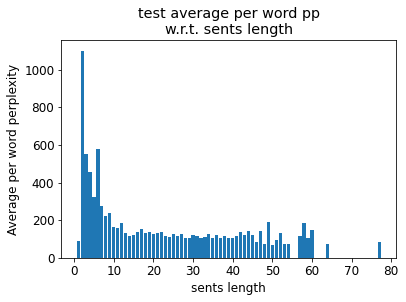
\includegraphics[scale=0.40]{assets/awdlstm_test_pp_per_length.png}
    \vspace{-1.0em}
    \caption{AWD-LSTM average perplexity per sentence length on the test set}
    \vspace{-1.0em}
    \label{fig:awdlstm-test-pp}
\end{figure}

Then, I looked at the average per word perplexity associated with sentences having a certain length. From this second analysis, a more interesting behaviour was discovered. \Cref{fig:baseline-train-pp} and \Cref{fig:baseline-test-pp} show its results on the baseline model on the train and test set respectively. From here we can observe two things: first of all, in both figures we can see that the model has a higher perplexity for shorter sentences; secondly, on the training set we also seem to have an issues with longer sentences.

Starting from the second issue, I decided to take a look at the results of the Baseline model that overfitted. In fact, I suspected that such behaviour was simply the result of a lack of training on the data, due to my early stopping criterion. In fact, by looking at \Cref{fig:overfit-train-pp} we can see that such behaviour has not completely disappeared, but has been greatly reduced. Moreover, another thing that can be considered is that the Baseline model has only a single recurrent layer and a limited embedding dimension, meaning that it can only capture context up to a certain length. Indeed, such behaviour is not present in AWD-LSTM.

Instead, shorter sentences seem to remain an issue even for AWD-LSTM, as shown in \Cref{fig:awdlstm-test-pp}. For this reason, I have decided to take a look at the word distribution that characterises sentences with at most 6 words. Thanks to such an analysis, I discovered why the model performed poorly: in fact, the most frequent words are the `\texttt{<unk>}' tag, the determinants, and the to be verb. This means that the possible continuations of sentences characterised by such words are extremely situational; meaning that the model can indeed find the best follow-up word for the training set by overfitting; but, it will have no chance of reaching good performance on the validation and test data if such follow-ups do not hold anymore.
